%%%%%%%%%%%%%%%%%%%%%%%%%%%%%%%%%%%%%%%%%%%%%%%%%%%%%%%%%%%%%%%%%%%%%%%%%%%
%% This file is part of the book
%%
%% Algorithmic Graph Theory
%% http://code.google.com/p/graph-theory-algorithms-book/
%%
%% Copyright (C) 2009, 2010, 2011 Minh Van Nguyen <nguyenminh2@gmail.com>
%%
%% See the file COPYING for copying conditions.
%%%%%%%%%%%%%%%%%%%%%%%%%%%%%%%%%%%%%%%%%%%%%%%%%%%%%%%%%%%%%%%%%%%%%%%%%%%

\documentclass{article}

\usepackage{subfigure}
\usepackage{tikz}
\usetikzlibrary{external}
\tikzexternalize{binomial-random-graphs-25-nodes}

\begin{document}

\begin{figure}
\subfigure[$p = 0$;
  $\alpha = 0$, $|E| = 0$;
  $\beta = 0$, $\#\deg = 0$]{
\begin{tikzpicture}
[lineDecorate/.style={-,thick},%
  nodeDecorate/.style={shape=circle,inner sep=2pt,draw,thick},
  scale=3.4]
%% nodes or vertices
\foreach \nodename/\x/\y in {
  0/1.00000000000000/0.000000000000000,
  1/0.968583161128631/0.248689887164855,
  2/0.876306680043864/0.481753674101715,
  3/0.728968627421412/0.684547105928689,
  4/0.535826794978997/0.844327925502015,
  5/0.309016994374947/0.951056516295154,
  6/0.0627905195293135/0.998026728428272,
  7/-0.187381314585725/0.982287250728689,
  8/-0.425779291565073/0.904827052466019,
  9/-0.637423989748690/0.770513242775789,
  10/-0.809016994374947/0.587785252292473,
  11/-0.929776485888251/0.368124552684678,
  12/-0.992114701314478/0.125333233564305,
  13/-0.992114701314478/-0.125333233564304,
  14/-0.929776485888251/-0.368124552684678,
  15/-0.809016994374947/-0.587785252292473,
  16/-0.637423989748690/-0.770513242775789,
  17/-0.425779291565072/-0.904827052466020,
  18/-0.187381314585725/-0.982287250728689,
  19/0.0627905195293128/-0.998026728428272,
  20/0.309016994374947/-0.951056516295154,
  21/0.535826794978996/-0.844327925502016,
  22/0.728968627421411/-0.684547105928689,
  23/0.876306680043864/-0.481753674101715,
  24/0.968583161128631/-0.248689887164855}
{
  \node (\nodename) at (\x,\y) [nodeDecorate] {};
}
\end{tikzpicture}
}
%%
%%
\qquad
\subfigure[$p = 1/6$;
  $\alpha = 50$, $|E| = 44$;
  $\beta = 100$, $\#\deg = 88$]{
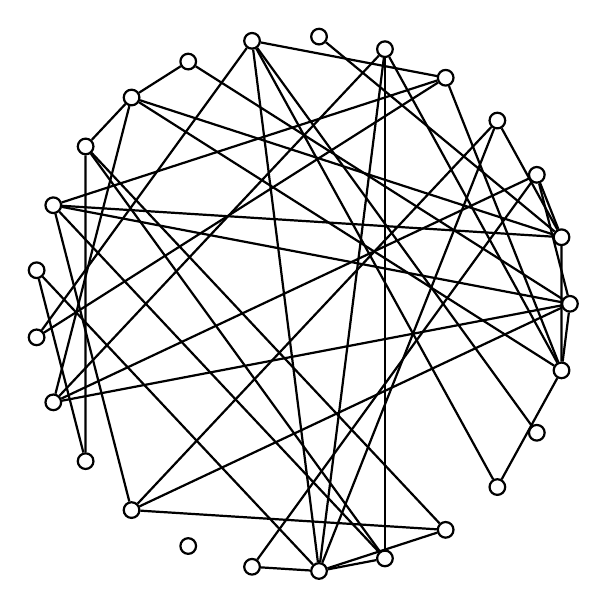
\begin{tikzpicture}
[lineDecorate/.style={-,thick},%
  nodeDecorate/.style={shape=circle,inner sep=2pt,draw,thick},
  scale=3.4]
%% nodes or vertices
\foreach \nodename/\x/\y in {
  0/1.00000000000000/0.000000000000000,
  1/0.968583161128631/0.248689887164855,
  2/0.876306680043864/0.481753674101715,
  3/0.728968627421412/0.684547105928689,
  4/0.535826794978997/0.844327925502015,
  5/0.309016994374947/0.951056516295154,
  6/0.0627905195293135/0.998026728428272,
  7/-0.187381314585725/0.982287250728689,
  8/-0.425779291565073/0.904827052466019,
  9/-0.637423989748690/0.770513242775789,
  10/-0.809016994374947/0.587785252292473,
  11/-0.929776485888251/0.368124552684678,
  12/-0.992114701314478/0.125333233564305,
  13/-0.992114701314478/-0.125333233564304,
  14/-0.929776485888251/-0.368124552684678,
  15/-0.809016994374947/-0.587785252292473,
  16/-0.637423989748690/-0.770513242775789,
  17/-0.425779291565072/-0.904827052466020,
  18/-0.187381314585725/-0.982287250728689,
  19/0.0627905195293128/-0.998026728428272,
  20/0.309016994374947/-0.951056516295154,
  21/0.535826794978996/-0.844327925502016,
  22/0.728968627421411/-0.684547105928689,
  23/0.876306680043864/-0.481753674101715,
  24/0.968583161128631/-0.248689887164855}
{
  \node (\nodename) at (\x,\y) [nodeDecorate] {};
}
%% edges or lines
\path
\foreach \startnode/\endnode in {
  0/2, 0/8, 0/11, 0/14, 0/16, 0/24, 1/2, 1/3, 1/6, 1/9, 1/11, 1/24,
  2/14, 2/18, 3/16, 3/19, 4/7, 4/11, 4/13, 4/24, 5/14, 5/19, 5/20, 5/24,
  7/13, 7/19, 7/22, 7/23, 8/9, 9/10, 9/14, 9/24, 10/15, 10/20, 10/21,
  11/16, 11/20, 12/15, 12/19, 16/21, 18/19, 19/20, 19/21, 22/24}
{
  (\startnode) edge[lineDecorate] node {} (\endnode)
};
\end{tikzpicture}
}
%%
%%
\subfigure[$p = 1/3$;
  $\alpha = 100$, $|E| = 108$;
  $\beta = 200$, $\#\deg = 212$]{
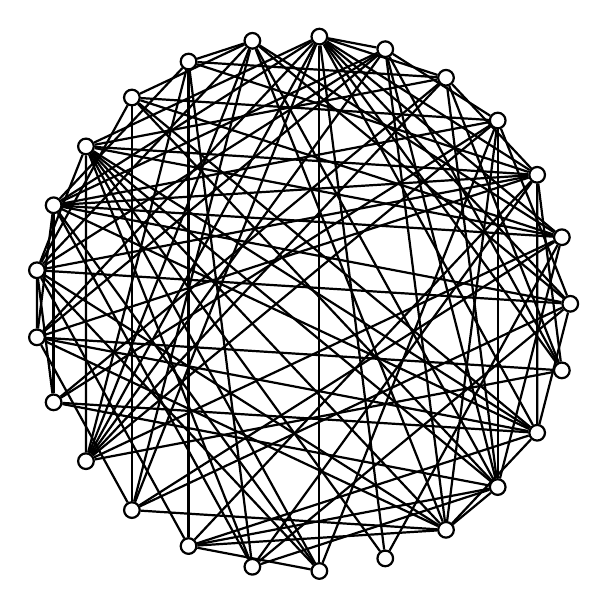
\begin{tikzpicture}
[lineDecorate/.style={-,thick},%
  nodeDecorate/.style={shape=circle,inner sep=2pt,draw,thick},
  scale=3.4]
%% nodes or vertices
\foreach \nodename/\x/\y in {
  0/1.00000000000000/0.000000000000000,
  1/0.968583161128631/0.248689887164855,
  2/0.876306680043864/0.481753674101715,
  3/0.728968627421412/0.684547105928689,
  4/0.535826794978997/0.844327925502015,
  5/0.309016994374947/0.951056516295154,
  6/0.0627905195293135/0.998026728428272,
  7/-0.187381314585725/0.982287250728689,
  8/-0.425779291565073/0.904827052466019,
  9/-0.637423989748690/0.770513242775789,
  10/-0.809016994374947/0.587785252292473,
  11/-0.929776485888251/0.368124552684678,
  12/-0.992114701314478/0.125333233564305,
  13/-0.992114701314478/-0.125333233564304,
  14/-0.929776485888251/-0.368124552684678,
  15/-0.809016994374947/-0.587785252292473,
  16/-0.637423989748690/-0.770513242775789,
  17/-0.425779291565072/-0.904827052466020,
  18/-0.187381314585725/-0.982287250728689,
  19/0.0627905195293128/-0.998026728428272,
  20/0.309016994374947/-0.951056516295154,
  21/0.535826794978996/-0.844327925502016,
  22/0.728968627421411/-0.684547105928689,
  23/0.876306680043864/-0.481753674101715,
  24/0.968583161128631/-0.248689887164855}
{
  \node (\nodename) at (\x,\y) [nodeDecorate] {};
}
%% edges or lines
\path
\foreach \startnode/\endnode in {
  0/3, 0/6, 0/7, 0/11, 0/12, 0/16, 0/18, 0/23, 1/6, 1/7, 1/9, 1/10,
  1/11, 1/15, 1/16, 1/20, 1/22, 2/4, 2/6, 2/8, 2/10, 2/11, 2/12, 2/13,
  2/17, 2/18, 2/23, 2/24, 3/5, 3/9, 3/11, 3/14, 3/15, 3/19, 3/21, 3/22,
  4/6, 4/8, 4/10, 4/14, 4/15, 4/22, 4/24, 5/6, 5/11, 5/12, 5/13, 5/15,
  5/21, 5/22, 5/24, 6/10, 6/11, 6/13, 6/15, 6/16, 6/19, 6/20, 6/23,
  6/24, 7/8, 7/9, 7/12, 7/15, 7/16, 7/21, 7/22, 8/11, 8/15, 8/17, 8/18,
  9/12, 9/16, 9/22, 9/23, 10/12, 10/15, 10/18, 10/19, 10/20, 10/21,
  10/22, 10/23, 11/13, 11/14, 11/18, 11/19, 11/23, 12/13, 12/14, 12/17,
  12/19, 12/21, 13/16, 13/21, 13/23, 13/24, 14/22, 14/23, 15/24, 16/21,
  17/19, 17/21, 17/22, 17/23, 18/22, 21/22, 21/23}
{
  (\startnode) edge[lineDecorate] node {} (\endnode)
};
\end{tikzpicture}
}
%%
%%
\qquad
\subfigure[$p = 1/2$;
  $\alpha = 150$, $|E| = 156$;
  $\beta = 300$, $\#\deg = 312$]{
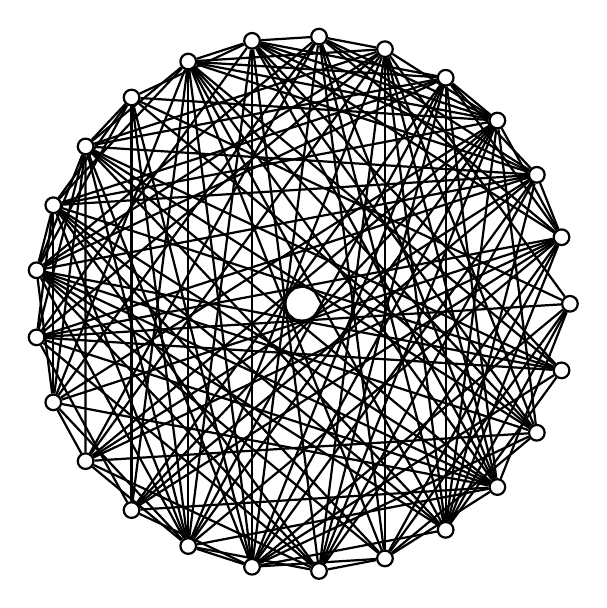
\begin{tikzpicture}
[lineDecorate/.style={-,thick},%
  nodeDecorate/.style={shape=circle,inner sep=2pt,draw,thick},
  scale=3.4]
%% nodes or vertices
\foreach \nodename/\x/\y in {
  0/1.00000000000000/0.000000000000000,
  1/0.968583161128631/0.248689887164855,
  2/0.876306680043864/0.481753674101715,
  3/0.728968627421412/0.684547105928689,
  4/0.535826794978997/0.844327925502015,
  5/0.309016994374947/0.951056516295154,
  6/0.0627905195293135/0.998026728428272,
  7/-0.187381314585725/0.982287250728689,
  8/-0.425779291565073/0.904827052466019,
  9/-0.637423989748690/0.770513242775789,
  10/-0.809016994374947/0.587785252292473,
  11/-0.929776485888251/0.368124552684678,
  12/-0.992114701314478/0.125333233564305,
  13/-0.992114701314478/-0.125333233564304,
  14/-0.929776485888251/-0.368124552684678,
  15/-0.809016994374947/-0.587785252292473,
  16/-0.637423989748690/-0.770513242775789,
  17/-0.425779291565072/-0.904827052466020,
  18/-0.187381314585725/-0.982287250728689,
  19/0.0627905195293128/-0.998026728428272,
  20/0.309016994374947/-0.951056516295154,
  21/0.535826794978996/-0.844327925502016,
  22/0.728968627421411/-0.684547105928689,
  23/0.876306680043864/-0.481753674101715,
  24/0.968583161128631/-0.248689887164855}
{
  \node (\nodename) at (\x,\y) [nodeDecorate] {};
}
%% edges or lines
\path
\foreach \startnode/\endnode in {
  0/5, 0/9, 0/13, 0/18, 0/20, 0/21, 0/22, 1/2, 1/3, 1/4, 1/6, 1/7, 1/13,
  1/14, 1/15, 1/16, 1/17, 1/19, 1/20, 1/21, 2/4, 2/6, 2/7, 2/8, 2/10,
  2/11, 2/12, 2/13, 2/15, 2/16, 2/18, 2/19, 2/21, 3/4, 3/5, 3/6, 3/7,
  3/8, 3/9, 3/11, 3/14, 3/15, 3/16, 3/17, 3/18, 3/19, 3/21, 3/23, 4/7,
  4/8, 4/10, 4/11, 4/12, 4/16, 4/17, 4/18, 4/19, 4/21, 4/22, 5/6, 5/8,
  5/10, 5/12, 5/13, 5/15, 5/17, 5/19, 5/20, 5/21, 5/22, 5/23, 6/7, 6/12,
  6/14, 6/15, 6/18, 6/20, 6/21, 6/22, 7/8, 7/9, 7/13, 7/17, 7/18, 7/19,
  7/22, 7/23, 7/24, 8/10, 8/11, 8/14, 8/16, 8/17, 8/18, 8/20, 8/21,
  8/22, 8/23, 8/24, 9/10, 9/11, 9/12, 9/16, 9/17, 9/18, 9/23, 10/12,
  10/13, 10/14, 10/15, 10/17, 10/18, 10/21, 10/22, 10/23, 10/24, 11/12,
  11/13, 11/14, 11/17, 11/19, 11/20, 11/21, 11/22, 11/24, 12/14, 12/17,
  12/19, 12/20, 12/21, 12/22, 12/23, 12/24, 13/16, 13/19, 13/22, 13/24,
  14/15, 14/17, 14/22, 15/17, 15/19, 15/23, 16/18, 16/22, 17/18, 17/19,
  17/22, 18/20, 18/21, 18/23, 18/24, 19/20, 20/22, 20/23, 21/24}
{
  (\startnode) edge[lineDecorate] node {} (\endnode)
};
\end{tikzpicture}
}
%%
%%
\subfigure[$p = 2/3$;
  $\alpha = 200$, $|E| = 185$;
  $\beta = 400$, $\#\deg = 370$]{
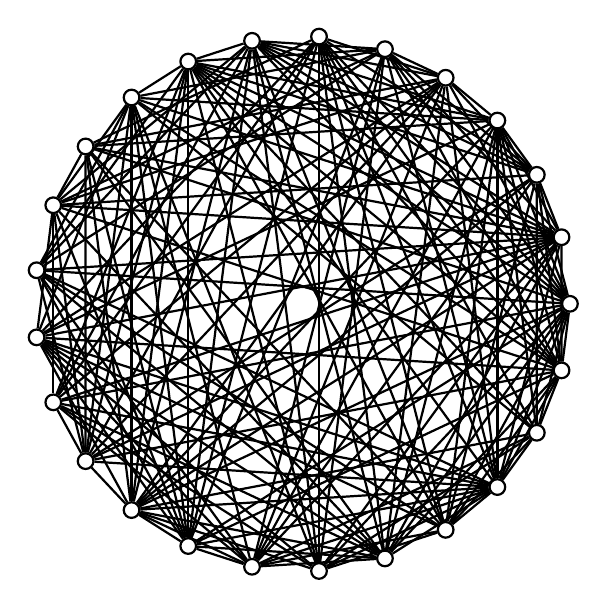
\begin{tikzpicture}
[lineDecorate/.style={-,thick},%
  nodeDecorate/.style={shape=circle,inner sep=2pt,draw,thick},
  scale=3.4]
%% nodes or vertices
\foreach \nodename/\x/\y in {
  0/1.00000000000000/0.000000000000000,
  1/0.968583161128631/0.248689887164855,
  2/0.876306680043864/0.481753674101715,
  3/0.728968627421412/0.684547105928689,
  4/0.535826794978997/0.844327925502015,
  5/0.309016994374947/0.951056516295154,
  6/0.0627905195293135/0.998026728428272,
  7/-0.187381314585725/0.982287250728689,
  8/-0.425779291565073/0.904827052466019,
  9/-0.637423989748690/0.770513242775789,
  10/-0.809016994374947/0.587785252292473,
  11/-0.929776485888251/0.368124552684678,
  12/-0.992114701314478/0.125333233564305,
  13/-0.992114701314478/-0.125333233564304,
  14/-0.929776485888251/-0.368124552684678,
  15/-0.809016994374947/-0.587785252292473,
  16/-0.637423989748690/-0.770513242775789,
  17/-0.425779291565072/-0.904827052466020,
  18/-0.187381314585725/-0.982287250728689,
  19/0.0627905195293128/-0.998026728428272,
  20/0.309016994374947/-0.951056516295154,
  21/0.535826794978996/-0.844327925502016,
  22/0.728968627421411/-0.684547105928689,
  23/0.876306680043864/-0.481753674101715,
  24/0.968583161128631/-0.248689887164855}
{
  \node (\nodename) at (\x,\y) [nodeDecorate] {};
}
%% edges or lines
\path
\foreach \startnode/\endnode in {
  0/2, 0/3, 0/4, 0/5, 0/6, 0/7, 0/8, 0/10, 0/12, 0/14, 0/16, 0/17, 0/19,
  0/20, 0/21, 0/22, 0/23, 0/24, 1/2, 1/3, 1/5, 1/7, 1/8, 1/9, 1/10,
  1/11, 1/12, 1/13, 1/14, 1/15, 1/16, 1/18, 1/19, 1/20, 1/22, 1/24, 2/3,
  2/4, 2/5, 2/6, 2/7, 2/8, 2/11, 2/15, 2/16, 2/18, 2/21, 2/23, 2/24,
  3/4, 3/7, 3/8, 3/9, 3/10, 3/13, 3/16, 3/18, 3/20, 3/21, 3/22, 3/23,
  3/24, 4/5, 4/6, 4/7, 4/10, 4/11, 4/13, 4/14, 4/15, 4/16, 4/18, 4/20,
  4/22, 5/7, 5/8, 5/9, 5/11, 5/12, 5/17, 5/18, 5/19, 5/22, 5/24, 6/10,
  6/13, 6/14, 6/15, 6/17, 6/19, 6/20, 6/21, 6/22, 6/23, 6/24, 7/8, 7/11,
  7/12, 7/14, 7/16, 7/17, 7/19, 7/20, 7/21, 7/24, 8/9, 8/12, 8/14, 8/15,
  8/16, 8/17, 8/19, 8/21, 8/22, 8/23, 8/24, 9/11, 9/12, 9/13, 9/15,
  9/16, 9/17, 9/18, 9/19, 9/23, 9/24, 10/11, 10/15, 10/16, 10/17, 10/20,
  10/21, 11/13, 11/14, 11/15, 11/17, 11/20, 11/24, 12/15, 12/17, 12/18,
  12/20, 12/21, 12/22, 13/16, 13/17, 13/18, 13/19, 13/20, 13/21, 13/22,
  13/24, 14/15, 14/18, 14/19, 14/20, 14/22, 15/16, 15/22, 15/24, 16/17,
  16/18, 16/19, 16/20, 16/22, 16/23, 17/18, 17/20, 17/22, 17/24, 18/20,
  18/21, 18/22, 18/23, 19/21, 19/22, 19/23, 20/22, 20/24, 21/22, 21/23,
  21/24, 22/23, 22/24, 23/24}
{
  (\startnode) edge[lineDecorate] node {} (\endnode)
};
\end{tikzpicture}
}
%%
%%
\qquad
\subfigure[$p = 5/6$;
  $\alpha = 250$, $|E| = 255$;
  $\beta = 500$, $\#\deg = 510$]{
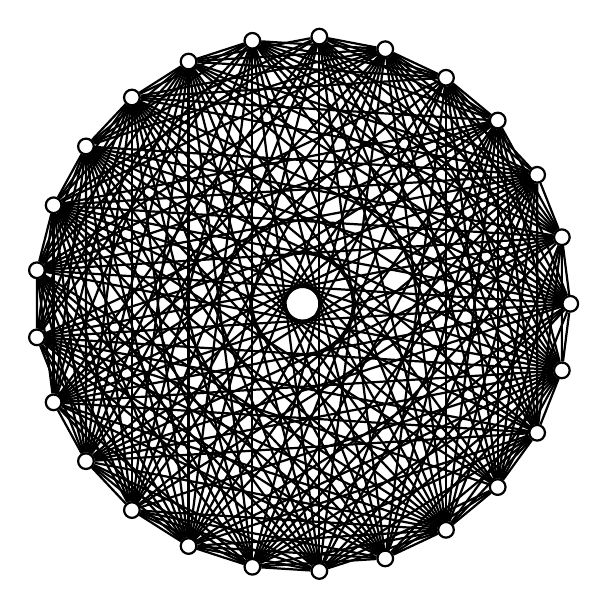
\begin{tikzpicture}
[lineDecorate/.style={-,thick},%
  nodeDecorate/.style={shape=circle,inner sep=2pt,draw,thick},
  scale=3.4]
%% nodes or vertices
\foreach \nodename/\x/\y in {
  0/1.00000000000000/0.000000000000000,
  1/0.968583161128631/0.248689887164855,
  2/0.876306680043864/0.481753674101715,
  3/0.728968627421412/0.684547105928689,
  4/0.535826794978997/0.844327925502015,
  5/0.309016994374947/0.951056516295154,
  6/0.0627905195293135/0.998026728428272,
  7/-0.187381314585725/0.982287250728689,
  8/-0.425779291565073/0.904827052466019,
  9/-0.637423989748690/0.770513242775789,
  10/-0.809016994374947/0.587785252292473,
  11/-0.929776485888251/0.368124552684678,
  12/-0.992114701314478/0.125333233564305,
  13/-0.992114701314478/-0.125333233564304,
  14/-0.929776485888251/-0.368124552684678,
  15/-0.809016994374947/-0.587785252292473,
  16/-0.637423989748690/-0.770513242775789,
  17/-0.425779291565072/-0.904827052466020,
  18/-0.187381314585725/-0.982287250728689,
  19/0.0627905195293128/-0.998026728428272,
  20/0.309016994374947/-0.951056516295154,
  21/0.535826794978996/-0.844327925502016,
  22/0.728968627421411/-0.684547105928689,
  23/0.876306680043864/-0.481753674101715,
  24/0.968583161128631/-0.248689887164855}
{
  \node (\nodename) at (\x,\y) [nodeDecorate] {};
}
%% edges or lines
\path
\foreach \startnode/\endnode in {
  0/1, 0/3, 0/4, 0/5, 0/6, 0/7, 0/8, 0/9, 0/10, 0/11, 0/12, 0/13, 0/14,
  0/15, 0/17, 0/18, 0/19, 0/22, 0/24, 1/2, 1/3, 1/4, 1/5, 1/6, 1/7, 1/8,
  1/10, 1/11, 1/12, 1/13, 1/14, 1/15, 1/16, 1/18, 1/21, 1/22, 1/23,
  1/24, 2/4, 2/5, 2/7, 2/8, 2/9, 2/10, 2/11, 2/12, 2/13, 2/14, 2/15,
  2/16, 2/17, 2/18, 2/19, 2/20, 2/21, 2/22, 2/23, 3/4, 3/5, 3/6, 3/7,
  3/9, 3/11, 3/12, 3/13, 3/14, 3/15, 3/17, 3/18, 3/19, 3/20, 3/21, 3/22,
  3/23, 3/24, 4/5, 4/6, 4/7, 4/8, 4/9, 4/12, 4/14, 4/16, 4/17, 4/18,
  4/20, 4/21, 4/22, 4/23, 4/24, 5/6, 5/7, 5/8, 5/9, 5/10, 5/11, 5/12,
  5/14, 5/15, 5/16, 5/17, 5/18, 5/19, 5/21, 5/22, 5/23, 5/24, 6/8, 6/10,
  6/11, 6/14, 6/15, 6/16, 6/17, 6/19, 6/20, 6/21, 6/22, 6/23, 6/24, 7/8,
  7/9, 7/10, 7/12, 7/13, 7/15, 7/16, 7/17, 7/18, 7/19, 7/20, 7/21, 7/23,
  7/24, 8/9, 8/10, 8/11, 8/12, 8/13, 8/14, 8/15, 8/16, 8/17, 8/18, 8/19,
  8/20, 8/21, 8/22, 8/24, 9/10, 9/11, 9/12, 9/13, 9/14, 9/15, 9/16,
  9/17, 9/18, 9/19, 9/20, 9/21, 9/22, 9/23, 9/24, 10/11, 10/12, 10/13,
  10/14, 10/15, 10/16, 10/17, 10/18, 10/19, 10/20, 10/21, 10/22, 10/23,
  10/24, 11/12, 11/13, 11/14, 11/15, 11/16, 11/17, 11/18, 11/19, 11/20,
  11/21, 11/22, 11/23, 11/24, 12/13, 12/14, 12/15, 12/16, 12/17, 12/18,
  12/19, 12/20, 12/21, 12/24, 13/15, 13/16, 13/17, 13/19, 13/20, 13/21,
  13/22, 13/23, 13/24, 14/15, 14/17, 14/18, 14/20, 14/21, 14/23, 14/24,
  15/16, 15/17, 15/18, 15/19, 15/21, 15/23, 15/24, 16/17, 16/18, 16/19,
  16/20, 16/21, 16/24, 17/18, 17/19, 17/20, 17/21, 17/23, 17/24, 18/19,
  18/20, 18/21, 18/23, 18/24, 19/21, 19/22, 19/23, 19/24, 20/21, 20/22,
  20/23, 20/24, 21/22, 21/23, 21/24, 22/23, 22/24, 23/24}
{
  (\startnode) edge[lineDecorate] node {} (\endnode)
};
\end{tikzpicture}
}
\end{figure}

\end{document}
